% Options for packages loaded elsewhere
\PassOptionsToPackage{unicode}{hyperref}
\PassOptionsToPackage{hyphens}{url}
%
\documentclass[
]{article}
\usepackage{amsmath,amssymb}
\usepackage{lmodern}
\usepackage{iftex}
\ifPDFTeX
  \usepackage[T1]{fontenc}
  \usepackage[utf8]{inputenc}
  \usepackage{textcomp} % provide euro and other symbols
\else % if luatex or xetex
  \usepackage{unicode-math}
  \defaultfontfeatures{Scale=MatchLowercase}
  \defaultfontfeatures[\rmfamily]{Ligatures=TeX,Scale=1}
\fi
% Use upquote if available, for straight quotes in verbatim environments
\IfFileExists{upquote.sty}{\usepackage{upquote}}{}
\IfFileExists{microtype.sty}{% use microtype if available
  \usepackage[]{microtype}
  \UseMicrotypeSet[protrusion]{basicmath} % disable protrusion for tt fonts
}{}
\makeatletter
\@ifundefined{KOMAClassName}{% if non-KOMA class
  \IfFileExists{parskip.sty}{%
    \usepackage{parskip}
  }{% else
    \setlength{\parindent}{0pt}
    \setlength{\parskip}{6pt plus 2pt minus 1pt}}
}{% if KOMA class
  \KOMAoptions{parskip=half}}
\makeatother
\usepackage{xcolor}
\usepackage[margin=1in]{geometry}
\usepackage{color}
\usepackage{fancyvrb}
\newcommand{\VerbBar}{|}
\newcommand{\VERB}{\Verb[commandchars=\\\{\}]}
\DefineVerbatimEnvironment{Highlighting}{Verbatim}{commandchars=\\\{\}}
% Add ',fontsize=\small' for more characters per line
\usepackage{framed}
\definecolor{shadecolor}{RGB}{248,248,248}
\newenvironment{Shaded}{\begin{snugshade}}{\end{snugshade}}
\newcommand{\AlertTok}[1]{\textcolor[rgb]{0.94,0.16,0.16}{#1}}
\newcommand{\AnnotationTok}[1]{\textcolor[rgb]{0.56,0.35,0.01}{\textbf{\textit{#1}}}}
\newcommand{\AttributeTok}[1]{\textcolor[rgb]{0.77,0.63,0.00}{#1}}
\newcommand{\BaseNTok}[1]{\textcolor[rgb]{0.00,0.00,0.81}{#1}}
\newcommand{\BuiltInTok}[1]{#1}
\newcommand{\CharTok}[1]{\textcolor[rgb]{0.31,0.60,0.02}{#1}}
\newcommand{\CommentTok}[1]{\textcolor[rgb]{0.56,0.35,0.01}{\textit{#1}}}
\newcommand{\CommentVarTok}[1]{\textcolor[rgb]{0.56,0.35,0.01}{\textbf{\textit{#1}}}}
\newcommand{\ConstantTok}[1]{\textcolor[rgb]{0.00,0.00,0.00}{#1}}
\newcommand{\ControlFlowTok}[1]{\textcolor[rgb]{0.13,0.29,0.53}{\textbf{#1}}}
\newcommand{\DataTypeTok}[1]{\textcolor[rgb]{0.13,0.29,0.53}{#1}}
\newcommand{\DecValTok}[1]{\textcolor[rgb]{0.00,0.00,0.81}{#1}}
\newcommand{\DocumentationTok}[1]{\textcolor[rgb]{0.56,0.35,0.01}{\textbf{\textit{#1}}}}
\newcommand{\ErrorTok}[1]{\textcolor[rgb]{0.64,0.00,0.00}{\textbf{#1}}}
\newcommand{\ExtensionTok}[1]{#1}
\newcommand{\FloatTok}[1]{\textcolor[rgb]{0.00,0.00,0.81}{#1}}
\newcommand{\FunctionTok}[1]{\textcolor[rgb]{0.00,0.00,0.00}{#1}}
\newcommand{\ImportTok}[1]{#1}
\newcommand{\InformationTok}[1]{\textcolor[rgb]{0.56,0.35,0.01}{\textbf{\textit{#1}}}}
\newcommand{\KeywordTok}[1]{\textcolor[rgb]{0.13,0.29,0.53}{\textbf{#1}}}
\newcommand{\NormalTok}[1]{#1}
\newcommand{\OperatorTok}[1]{\textcolor[rgb]{0.81,0.36,0.00}{\textbf{#1}}}
\newcommand{\OtherTok}[1]{\textcolor[rgb]{0.56,0.35,0.01}{#1}}
\newcommand{\PreprocessorTok}[1]{\textcolor[rgb]{0.56,0.35,0.01}{\textit{#1}}}
\newcommand{\RegionMarkerTok}[1]{#1}
\newcommand{\SpecialCharTok}[1]{\textcolor[rgb]{0.00,0.00,0.00}{#1}}
\newcommand{\SpecialStringTok}[1]{\textcolor[rgb]{0.31,0.60,0.02}{#1}}
\newcommand{\StringTok}[1]{\textcolor[rgb]{0.31,0.60,0.02}{#1}}
\newcommand{\VariableTok}[1]{\textcolor[rgb]{0.00,0.00,0.00}{#1}}
\newcommand{\VerbatimStringTok}[1]{\textcolor[rgb]{0.31,0.60,0.02}{#1}}
\newcommand{\WarningTok}[1]{\textcolor[rgb]{0.56,0.35,0.01}{\textbf{\textit{#1}}}}
\usepackage{graphicx}
\makeatletter
\def\maxwidth{\ifdim\Gin@nat@width>\linewidth\linewidth\else\Gin@nat@width\fi}
\def\maxheight{\ifdim\Gin@nat@height>\textheight\textheight\else\Gin@nat@height\fi}
\makeatother
% Scale images if necessary, so that they will not overflow the page
% margins by default, and it is still possible to overwrite the defaults
% using explicit options in \includegraphics[width, height, ...]{}
\setkeys{Gin}{width=\maxwidth,height=\maxheight,keepaspectratio}
% Set default figure placement to htbp
\makeatletter
\def\fps@figure{htbp}
\makeatother
\setlength{\emergencystretch}{3em} % prevent overfull lines
\providecommand{\tightlist}{%
  \setlength{\itemsep}{0pt}\setlength{\parskip}{0pt}}
\setcounter{secnumdepth}{-\maxdimen} % remove section numbering
\ifLuaTeX
  \usepackage{selnolig}  % disable illegal ligatures
\fi
\IfFileExists{bookmark.sty}{\usepackage{bookmark}}{\usepackage{hyperref}}
\IfFileExists{xurl.sty}{\usepackage{xurl}}{} % add URL line breaks if available
\urlstyle{same} % disable monospaced font for URLs
\hypersetup{
  pdftitle={Untitled},
  hidelinks,
  pdfcreator={LaTeX via pandoc}}

\title{Untitled}
\author{}
\date{\vspace{-2.5em}2023-04-26}

\begin{document}
\maketitle

\begin{Shaded}
\begin{Highlighting}[]
\FunctionTok{library}\NormalTok{(dplyr)}
\end{Highlighting}
\end{Shaded}

\begin{verbatim}
## Warning: package 'dplyr' was built under R version 4.2.3
\end{verbatim}

\begin{verbatim}
## 
## Attaching package: 'dplyr'
\end{verbatim}

\begin{verbatim}
## The following objects are masked from 'package:stats':
## 
##     filter, lag
\end{verbatim}

\begin{verbatim}
## The following objects are masked from 'package:base':
## 
##     intersect, setdiff, setequal, union
\end{verbatim}

\begin{Shaded}
\begin{Highlighting}[]
\FunctionTok{library}\NormalTok{(readxl)}
\end{Highlighting}
\end{Shaded}

\begin{verbatim}
## Warning: package 'readxl' was built under R version 4.2.3
\end{verbatim}

\begin{Shaded}
\begin{Highlighting}[]
\NormalTok{gendergap }\OtherTok{\textless{}{-}} \FunctionTok{read\_excel}\NormalTok{(}\StringTok{"data/gendergap.xlsx"}\NormalTok{ , }\AttributeTok{skip =} \DecValTok{3}\NormalTok{)}
\FunctionTok{View}\NormalTok{(gendergap)}
\end{Highlighting}
\end{Shaded}

sadece male verileri

\begin{Shaded}
\begin{Highlighting}[]
\NormalTok{gendergap }\SpecialCharTok{\%\textgreater{}\%}
\FunctionTok{group\_by}\NormalTok{(Sex) }\SpecialCharTok{\%\textgreater{}\%}
  \FunctionTok{filter}\NormalTok{(Sex }\SpecialCharTok{!=} \StringTok{"Total"}\NormalTok{) }\SpecialCharTok{\%\textgreater{}\%}
\FunctionTok{filter}\NormalTok{(Sex }\SpecialCharTok{!=} \StringTok{"Female"}\NormalTok{)}
\end{Highlighting}
\end{Shaded}

\begin{verbatim}
## # A tibble: 504 x 19
## # Groups:   Sex [1]
##    Country     Sex    Time  Total Managers Professionals Technicians and assoc~1
##    <chr>       <chr> <dbl>  <dbl>    <dbl>         <dbl>                   <dbl>
##  1 Afghanistan Male   2014   53.7    101.           88.8                    87.1
##  2 Afghanistan Male   2020   59.3     96.0          91.2                    71.2
##  3 Albania     Male   2012 2409.    4924.         3282.                   3136. 
##  4 Albania     Male   2018  303      562           436                     361  
##  5 Angola      Male   2019  679.    1059.         1239.                   1268. 
##  6 Angola      Male   2021  574.     721.         1158.                    932. 
##  7 Argentina   Male   2011   19.6     43.2          35.7                    25.5
##  8 Argentina   Male   2012   24.6     51.2          44.6                    32.2
##  9 Argentina   Male   2013   31.6     63.8          59.7                    42.4
## 10 Argentina   Male   2014   40.9     84.7          74.8                    51.8
## # i 494 more rows
## # i abbreviated name: 1: `Technicians and associate professionals`
## # i 12 more variables: `Clerical support workers` <dbl>,
## #   `Service and sales workers` <dbl>,
## #   `Skilled agricultural, forestry and fishery workers` <dbl>,
## #   `Craft and related trades workers` <dbl>,
## #   `Plant and machine operators, and assemblers` <dbl>, ...
\end{verbatim}

sadece female verileri

\begin{Shaded}
\begin{Highlighting}[]
\FunctionTok{options}\NormalTok{(}\AttributeTok{repos =} \FunctionTok{list}\NormalTok{(}\AttributeTok{CRAN=}\StringTok{"http://cran.rstudio.com/"}\NormalTok{))}
\NormalTok{gendergap }\SpecialCharTok{\%\textgreater{}\%}
\FunctionTok{group\_by}\NormalTok{(Sex) }\SpecialCharTok{\%\textgreater{}\%}
  \FunctionTok{filter}\NormalTok{(Sex }\SpecialCharTok{!=} \StringTok{"Total"}\NormalTok{) }\SpecialCharTok{\%\textgreater{}\%}
\FunctionTok{filter}\NormalTok{(Sex}\SpecialCharTok{!=} \StringTok{"Male"}\NormalTok{)}
\end{Highlighting}
\end{Shaded}

\begin{verbatim}
## # A tibble: 504 x 19
## # Groups:   Sex [1]
##    Country     Sex     Time  Total Managers Professionals Technicians and asso~1
##    <chr>       <chr>  <dbl>  <dbl>    <dbl>         <dbl>                  <dbl>
##  1 Afghanistan Female  2014   49.8    120.           75.0                   78.2
##  2 Afghanistan Female  2020   39.8    116.           75.3                   85.9
##  3 Albania     Female  2012 2005.    3571.         2794.                  2034. 
##  4 Albania     Female  2018  282      581           376                    330  
##  5 Angola      Female  2019  500.    1062.         1101.                   740. 
##  6 Angola      Female  2021  501.    1414.         1179.                   816. 
##  7 Argentina   Female  2011   19.4     36.8          32.2                   24.0
##  8 Argentina   Female  2012   24.8     54.2          39.5                   29.4
##  9 Argentina   Female  2013   31.2     62.9          49.6                   37.9
## 10 Argentina   Female  2014   41.1     79.6          65.4                   49.2
## # i 494 more rows
## # i abbreviated name: 1: `Technicians and associate professionals`
## # i 12 more variables: `Clerical support workers` <dbl>,
## #   `Service and sales workers` <dbl>,
## #   `Skilled agricultural, forestry and fishery workers` <dbl>,
## #   `Craft and related trades workers` <dbl>,
## #   `Plant and machine operators, and assemblers` <dbl>, ...
\end{verbatim}

\begin{Shaded}
\begin{Highlighting}[]
\NormalTok{only\_male\_female }\OtherTok{\textless{}{-}}\NormalTok{ gendergap }\SpecialCharTok{\%\textgreater{}\%}
  \FunctionTok{filter}\NormalTok{(Sex }\SpecialCharTok{!=}\NormalTok{ Total)}

\NormalTok{only\_male\_female }\SpecialCharTok{\%\textgreater{}\%}
\NormalTok{  GGally}\SpecialCharTok{::}\FunctionTok{ggally\_box}\NormalTok{(}\AttributeTok{mapping =}\NormalTok{ ggplot2}\SpecialCharTok{::}\FunctionTok{aes}\NormalTok{(}\AttributeTok{x =}\NormalTok{ Total, }\AttributeTok{y =}\NormalTok{ Sex)) }\SpecialCharTok{+}
\NormalTok{  ggplot2}\SpecialCharTok{::}\FunctionTok{labs}\NormalTok{(}\AttributeTok{x =} \StringTok{""}\NormalTok{, }\AttributeTok{y =} \StringTok{""}\NormalTok{) }\SpecialCharTok{+}
\NormalTok{    ggplot2}\SpecialCharTok{::}\FunctionTok{theme\_minimal}\NormalTok{() }
\end{Highlighting}
\end{Shaded}

\begin{verbatim}
## Registered S3 method overwritten by 'GGally':
##   method from   
##   +.gg   ggplot2
\end{verbatim}

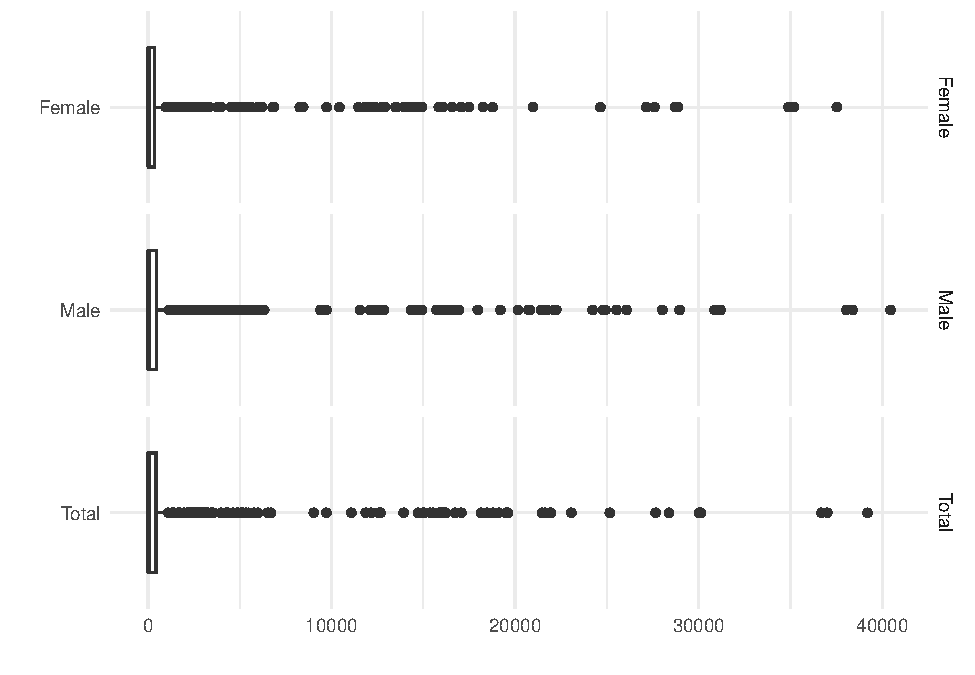
\includegraphics{Data-Analysis_files/figure-latex/unnamed-chunk-3-1.pdf}

\begin{Shaded}
\begin{Highlighting}[]
\NormalTok{gendergap }\SpecialCharTok{\%\textgreater{}\%}
\FunctionTok{filter}\NormalTok{(Sex }\SpecialCharTok{\%in\%} \FunctionTok{c}\NormalTok{(}\StringTok{"Male"}\NormalTok{, }\StringTok{"Female"}\NormalTok{)) }\SpecialCharTok{\%\textgreater{}\%}
\FunctionTok{t.test}\NormalTok{(Total }\SpecialCharTok{\textasciitilde{}}\NormalTok{ Sex, }\AttributeTok{data =}\NormalTok{ ., }\AttributeTok{alternative =} \StringTok{"two.sided"}\NormalTok{)}
\end{Highlighting}
\end{Shaded}

\begin{verbatim}
## 
##  Welch Two Sample t-test
## 
## data:  Total by Sex
## t = -0.70353, df = 989.27, p-value = 0.4819
## alternative hypothesis: true difference in means between group Female and group Male is not equal to 0
## 95 percent confidence interval:
##  -935.3974  441.6924
## sample estimates:
## mean in group Female   mean in group Male 
##             1853.069             2099.921
\end{verbatim}

ülkelere göre avg male earnings

\begin{Shaded}
\begin{Highlighting}[]
\NormalTok{gendergap }\SpecialCharTok{\%\textgreater{}\%}
  \FunctionTok{group\_by}\NormalTok{(Country) }\SpecialCharTok{\%\textgreater{}\%}
  \FunctionTok{filter}\NormalTok{(Sex }\SpecialCharTok{!=}\StringTok{"Total"}\NormalTok{) }\SpecialCharTok{\%\textgreater{}\%}
  \FunctionTok{filter}\NormalTok{(Sex }\SpecialCharTok{!=} \StringTok{"Female"}\NormalTok{) }\SpecialCharTok{\%\textgreater{}\%}
  \FunctionTok{summarise}\NormalTok{(}\AttributeTok{Male\_Avg\_Earngs =} \FunctionTok{mean}\NormalTok{(Total, }\AttributeTok{na.rm =} \ConstantTok{TRUE}\NormalTok{))}\SpecialCharTok{\%\textgreater{}\%}
  \FunctionTok{select}\NormalTok{(Country, Male\_Avg\_Earngs)}
\end{Highlighting}
\end{Shaded}

\begin{verbatim}
## # A tibble: 113 x 2
##    Country     Male_Avg_Earngs
##    <chr>                 <dbl>
##  1 Afghanistan           56.5 
##  2 Albania             1356.  
##  3 Angola               626.  
##  4 Argentina            126.  
##  5 Armenia              675.  
##  6 Austria               18.3 
##  7 Bangladesh            58.0 
##  8 Belarus                6.5 
##  9 Belgium               20.3 
## 10 Belize                 6.63
## # i 103 more rows
\end{verbatim}

ülkelere göre avg female earnings

\begin{Shaded}
\begin{Highlighting}[]
\NormalTok{gendergap }\SpecialCharTok{\%\textgreater{}\%}
  \FunctionTok{group\_by}\NormalTok{(Country) }\SpecialCharTok{\%\textgreater{}\%}
  \FunctionTok{filter}\NormalTok{(Sex }\SpecialCharTok{!=}\StringTok{"Total"}\NormalTok{) }\SpecialCharTok{\%\textgreater{}\%}
  \FunctionTok{filter}\NormalTok{(Sex }\SpecialCharTok{!=} \StringTok{"Male"}\NormalTok{) }\SpecialCharTok{\%\textgreater{}\%}
  \FunctionTok{summarise}\NormalTok{(}\AttributeTok{Female\_Avg\_Earngs =} \FunctionTok{mean}\NormalTok{(Total, }\AttributeTok{na.rm =} \ConstantTok{TRUE}\NormalTok{)) }\SpecialCharTok{\%\textgreater{}\%}
  \FunctionTok{select}\NormalTok{(Country, Female\_Avg\_Earngs) }
\end{Highlighting}
\end{Shaded}

\begin{verbatim}
## # A tibble: 113 x 2
##    Country     Female_Avg_Earngs
##    <chr>                   <dbl>
##  1 Afghanistan             44.8 
##  2 Albania               1143.  
##  3 Angola                 501.  
##  4 Argentina              125.  
##  5 Armenia                543.  
##  6 Austria                 14.4 
##  7 Bangladesh              53.3 
##  8 Belarus                  4.9 
##  9 Belgium                 18.2 
## 10 Belize                   7.23
## # i 103 more rows
\end{verbatim}

\begin{Shaded}
\begin{Highlighting}[]
  \FunctionTok{install.packages}\NormalTok{(}\StringTok{"ggplot2"}\NormalTok{)}
\end{Highlighting}
\end{Shaded}

\begin{verbatim}
## Installing package into 'C:/Users/sedau/AppData/Local/R/win-library/4.2'
## (as 'lib' is unspecified)
\end{verbatim}

\begin{verbatim}
## package 'ggplot2' successfully unpacked and MD5 sums checked
## 
## The downloaded binary packages are in
##  C:\Users\sedau\AppData\Local\Temp\RtmpMHO6Gv\downloaded_packages
\end{verbatim}

\begin{Shaded}
\begin{Highlighting}[]
\NormalTok{Average\_Earnings\_According\_to\_Sex\_And\_Country }\OtherTok{\textless{}{-}} \FunctionTok{aov}\NormalTok{(Total }\SpecialCharTok{\textasciitilde{}}\NormalTok{ Country }\SpecialCharTok{+}\NormalTok{ Sex, }\AttributeTok{data =}\NormalTok{ only\_male\_female)}
\NormalTok{broom}\SpecialCharTok{::}\FunctionTok{tidy}\NormalTok{(Average\_Earnings\_According\_to\_Sex\_And\_Country)  }
\end{Highlighting}
\end{Shaded}

\begin{verbatim}
## # A tibble: 3 x 6
##   term         df        sumsq     meansq statistic p.value
##   <chr>     <dbl>        <dbl>      <dbl>     <dbl>   <dbl>
## 1 Country     112 44759184367. 399635575.    233.    0     
## 2 Sex           2    15645290.   7822645.      4.57  0.0106
## 3 Residuals  1397  2393394045.   1713238.     NA    NA
\end{verbatim}

\begin{Shaded}
\begin{Highlighting}[]
\NormalTok{gendergap }\SpecialCharTok{\%\textgreater{}\%}
  \FunctionTok{filter}\NormalTok{(Country }\SpecialCharTok{==} \StringTok{"Afghanistan"}\NormalTok{) }\SpecialCharTok{\%\textgreater{}\%}
\FunctionTok{filter}\NormalTok{(Sex }\SpecialCharTok{\%in\%} \FunctionTok{c}\NormalTok{(}\StringTok{"Male"}\NormalTok{, }\StringTok{"Female"}\NormalTok{)) }\SpecialCharTok{\%\textgreater{}\%}
  \FunctionTok{t.test}\NormalTok{(Total }\SpecialCharTok{\textasciitilde{}}\NormalTok{ Sex, }\AttributeTok{data =}\NormalTok{., }\AttributeTok{alternative =} \StringTok{"two.sided"}\NormalTok{)}
\end{Highlighting}
\end{Shaded}

\begin{verbatim}
## 
##  Welch Two Sample t-test
## 
## data:  Total by Sex
## t = -2.0448, df = 1.583, p-value = 0.21
## alternative hypothesis: true difference in means between group Female and group Male is not equal to 0
## 95 percent confidence interval:
##  -43.8222  20.3622
## sample estimates:
## mean in group Female   mean in group Male 
##                44.78                56.51
\end{verbatim}

Tüm ülkelerdeki yıl bazında male avg earnings

\begin{Shaded}
\begin{Highlighting}[]
\NormalTok{gendergap }\SpecialCharTok{\%\textgreater{}\%}
  \FunctionTok{group\_by}\NormalTok{(Time) }\SpecialCharTok{\%\textgreater{}\%}
  \FunctionTok{filter}\NormalTok{(Sex }\SpecialCharTok{!=}\StringTok{"Total"}\NormalTok{) }\SpecialCharTok{\%\textgreater{}\%}
  \FunctionTok{filter}\NormalTok{(Sex }\SpecialCharTok{!=} \StringTok{"Female"}\NormalTok{) }\SpecialCharTok{\%\textgreater{}\%}
  \FunctionTok{arrange}\NormalTok{(Time) }\SpecialCharTok{\%\textgreater{}\%}
  \FunctionTok{mutate}\NormalTok{(}\AttributeTok{Male\_Avg\_Earngs =} \FunctionTok{mean}\NormalTok{(Total, }\AttributeTok{na.rm =} \ConstantTok{TRUE}\NormalTok{)) }\SpecialCharTok{\%\textgreater{}\%}
  \FunctionTok{select}\NormalTok{(Male\_Avg\_Earngs)}
\end{Highlighting}
\end{Shaded}

\begin{verbatim}
## Adding missing grouping variables: `Time`
\end{verbatim}

\begin{verbatim}
## # A tibble: 504 x 2
## # Groups:   Time [12]
##     Time Male_Avg_Earngs
##    <dbl>           <dbl>
##  1  2011           2847.
##  2  2011           2847.
##  3  2011           2847.
##  4  2011           2847.
##  5  2011           2847.
##  6  2011           2847.
##  7  2011           2847.
##  8  2011           2847.
##  9  2011           2847.
## 10  2011           2847.
## # i 494 more rows
\end{verbatim}

Tüm ülkelerdeki yıl bazında Female avg earnings

\begin{Shaded}
\begin{Highlighting}[]
\NormalTok{gendergap }\SpecialCharTok{\%\textgreater{}\%}
  \FunctionTok{group\_by}\NormalTok{(Time) }\SpecialCharTok{\%\textgreater{}\%}
  \FunctionTok{filter}\NormalTok{(Sex }\SpecialCharTok{!=}\StringTok{"Total"}\NormalTok{) }\SpecialCharTok{\%\textgreater{}\%}
  \FunctionTok{filter}\NormalTok{(Sex }\SpecialCharTok{!=} \StringTok{"Male"}\NormalTok{) }\SpecialCharTok{\%\textgreater{}\%}
  \FunctionTok{arrange}\NormalTok{(Time) }\SpecialCharTok{\%\textgreater{}\%}
  \FunctionTok{mutate}\NormalTok{(}\AttributeTok{Female\_Avg\_Earngs =} \FunctionTok{mean}\NormalTok{(Total, }\AttributeTok{na.rm =} \ConstantTok{TRUE}\NormalTok{)) }\SpecialCharTok{\%\textgreater{}\%}
  \FunctionTok{select}\NormalTok{(Female\_Avg\_Earngs )}
\end{Highlighting}
\end{Shaded}

\begin{verbatim}
## Adding missing grouping variables: `Time`
\end{verbatim}

\begin{verbatim}
## # A tibble: 504 x 2
## # Groups:   Time [12]
##     Time Female_Avg_Earngs
##    <dbl>             <dbl>
##  1  2011             2384.
##  2  2011             2384.
##  3  2011             2384.
##  4  2011             2384.
##  5  2011             2384.
##  6  2011             2384.
##  7  2011             2384.
##  8  2011             2384.
##  9  2011             2384.
## 10  2011             2384.
## # i 494 more rows
\end{verbatim}

\begin{Shaded}
\begin{Highlighting}[]
\NormalTok{devtools}\SpecialCharTok{::}\FunctionTok{install\_github}\NormalTok{(}\StringTok{"hrbrmstr/hrbrthemes"}\NormalTok{)}
\end{Highlighting}
\end{Shaded}

\begin{verbatim}
## Skipping install of 'hrbrthemes' from a github remote, the SHA1 (3e8d9494) has not changed since last install.
##   Use `force = TRUE` to force installation
\end{verbatim}

ülkelere göre female managers avg earnings

\begin{Shaded}
\begin{Highlighting}[]
\NormalTok{gendergap }\SpecialCharTok{\%\textgreater{}\%}
  \FunctionTok{group\_by}\NormalTok{(Country) }\SpecialCharTok{\%\textgreater{}\%} 
   \FunctionTok{filter}\NormalTok{(Sex }\SpecialCharTok{!=} \StringTok{"Total"}\NormalTok{) }\SpecialCharTok{\%\textgreater{}\%}
  \FunctionTok{filter}\NormalTok{(Sex }\SpecialCharTok{!=} \StringTok{"Male"}\NormalTok{) }\SpecialCharTok{\%\textgreater{}\%}
  \FunctionTok{summarise}\NormalTok{(}\AttributeTok{Female\_Managers\_Avg\_Earngs =} \FunctionTok{mean}\NormalTok{(Managers, }\AttributeTok{na.rm =} \ConstantTok{TRUE}\NormalTok{))}
\end{Highlighting}
\end{Shaded}

\begin{verbatim}
## # A tibble: 113 x 2
##    Country     Female_Managers_Avg_Earngs
##    <chr>                            <dbl>
##  1 Afghanistan                     118.  
##  2 Albania                        2076.  
##  3 Angola                         1238.  
##  4 Argentina                       254.  
##  5 Armenia                         835.  
##  6 Austria                          27.9 
##  7 Bangladesh                      140.  
##  8 Belarus                           7.24
##  9 Belgium                          34.3 
## 10 Belize                           11.9 
## # i 103 more rows
\end{verbatim}

ülkelere göre male managers avg earnings

\begin{Shaded}
\begin{Highlighting}[]
\NormalTok{gendergap }\SpecialCharTok{\%\textgreater{}\%}
  \FunctionTok{group\_by}\NormalTok{(Country) }\SpecialCharTok{\%\textgreater{}\%} 
   \FunctionTok{filter}\NormalTok{(Sex }\SpecialCharTok{!=} \StringTok{"Total"}\NormalTok{) }\SpecialCharTok{\%\textgreater{}\%}
  \FunctionTok{filter}\NormalTok{(Sex }\SpecialCharTok{!=} \StringTok{"Female"}\NormalTok{) }\SpecialCharTok{\%\textgreater{}\%}
  \FunctionTok{summarise}\NormalTok{(}\AttributeTok{Male\_Managers\_Avg\_Earngs =} \FunctionTok{mean}\NormalTok{(Managers, }\AttributeTok{na.rm =} \ConstantTok{TRUE}\NormalTok{))}
\end{Highlighting}
\end{Shaded}

\begin{verbatim}
## # A tibble: 113 x 2
##    Country     Male_Managers_Avg_Earngs
##    <chr>                          <dbl>
##  1 Afghanistan                    98.3 
##  2 Albania                      2743.  
##  3 Angola                        890.  
##  4 Argentina                     302.  
##  5 Armenia                      1003.  
##  6 Austria                        38.0 
##  7 Bangladesh                    130.  
##  8 Belarus                         9.98
##  9 Belgium                        39.4 
## 10 Belize                         11.3 
## # i 103 more rows
\end{verbatim}

ülkelere göre male professionals avg earnings

\begin{Shaded}
\begin{Highlighting}[]
\NormalTok{gendergap }\SpecialCharTok{\%\textgreater{}\%}
  \FunctionTok{group\_by}\NormalTok{(Country) }\SpecialCharTok{\%\textgreater{}\%} 
   \FunctionTok{filter}\NormalTok{(Sex }\SpecialCharTok{!=} \StringTok{"Total"}\NormalTok{) }\SpecialCharTok{\%\textgreater{}\%}
  \FunctionTok{filter}\NormalTok{(Sex }\SpecialCharTok{!=} \StringTok{"Female"}\NormalTok{) }\SpecialCharTok{\%\textgreater{}\%}
  \FunctionTok{summarise}\NormalTok{(}\AttributeTok{Male\_Professionals\_Avg\_Earngs =} \FunctionTok{mean}\NormalTok{(Professionals, }\AttributeTok{na.rm =} \ConstantTok{TRUE}\NormalTok{))}
\end{Highlighting}
\end{Shaded}

\begin{verbatim}
## # A tibble: 113 x 2
##    Country     Male_Professionals_Avg_Earngs
##    <chr>                               <dbl>
##  1 Afghanistan                          90.0
##  2 Albania                            1859. 
##  3 Angola                             1198. 
##  4 Argentina                           221. 
##  5 Armenia                             943. 
##  6 Austria                              26.1
##  7 Bangladesh                          127. 
##  8 Belarus                              11.2
##  9 Belgium                              27.1
## 10 Belize                               12.5
## # i 103 more rows
\end{verbatim}

ülkelere göre female professionals avg earnings

\begin{Shaded}
\begin{Highlighting}[]
\NormalTok{gendergap }\SpecialCharTok{\%\textgreater{}\%}
  \FunctionTok{group\_by}\NormalTok{(Country) }\SpecialCharTok{\%\textgreater{}\%} 
   \FunctionTok{filter}\NormalTok{(Sex }\SpecialCharTok{!=} \StringTok{"Total"}\NormalTok{) }\SpecialCharTok{\%\textgreater{}\%}
  \FunctionTok{filter}\NormalTok{(Sex }\SpecialCharTok{!=} \StringTok{"Male"}\NormalTok{) }\SpecialCharTok{\%\textgreater{}\%}
  \FunctionTok{summarise}\NormalTok{(}\AttributeTok{Female\_Professionals\_Avg\_Earngs =} \FunctionTok{mean}\NormalTok{(Professionals, }\AttributeTok{na.rm =} \ConstantTok{TRUE}\NormalTok{))}
\end{Highlighting}
\end{Shaded}

\begin{verbatim}
## # A tibble: 113 x 2
##    Country     Female_Professionals_Avg_Earngs
##    <chr>                                 <dbl>
##  1 Afghanistan                           75.2 
##  2 Albania                             1585.  
##  3 Angola                              1140.  
##  4 Argentina                            190.  
##  5 Armenia                              713.  
##  6 Austria                               21.3 
##  7 Bangladesh                           105.  
##  8 Belarus                                6.83
##  9 Belgium                               25.3 
## 10 Belize                                13.2 
## # i 103 more rows
\end{verbatim}

ülkelere göre Male technicians and associate professionals Avg Earngs

\begin{Shaded}
\begin{Highlighting}[]
\NormalTok{gendergap }\SpecialCharTok{\%\textgreater{}\%}
\NormalTok{  janitor}\SpecialCharTok{::}\FunctionTok{clean\_names}\NormalTok{() }\SpecialCharTok{\%\textgreater{}\%}
  \FunctionTok{group\_by}\NormalTok{(country) }\SpecialCharTok{\%\textgreater{}\%} 
  \FunctionTok{filter}\NormalTok{(sex }\SpecialCharTok{!=} \StringTok{"Total"}\NormalTok{) }\SpecialCharTok{\%\textgreater{}\%}
  \FunctionTok{filter}\NormalTok{(sex }\SpecialCharTok{!=} \StringTok{"Female"}\NormalTok{) }\SpecialCharTok{\%\textgreater{}\%}
  \FunctionTok{summarise}\NormalTok{(}\AttributeTok{Male\_technicians\_and\_associate\_professionals\_Avg\_Earngs =} \FunctionTok{mean}\NormalTok{(technicians\_and\_associate\_professionals, }\AttributeTok{na.rm =} \ConstantTok{TRUE}\NormalTok{))}
\end{Highlighting}
\end{Shaded}

\begin{verbatim}
## # A tibble: 113 x 2
##    country     Male_technicians_and_associate_professionals_Avg_Earngs
##    <chr>                                                         <dbl>
##  1 Afghanistan                                                   79.2 
##  2 Albania                                                     1748.  
##  3 Angola                                                      1100.  
##  4 Argentina                                                    168.  
##  5 Armenia                                                      710.  
##  6 Austria                                                       20.8 
##  7 Bangladesh                                                    86.8 
##  8 Belarus                                                        7.58
##  9 Belgium                                                       21.4 
## 10 Belize                                                        12.9 
## # i 103 more rows
\end{verbatim}

ülkelere göre female technicians and associate professionals Avg Earngs

\begin{Shaded}
\begin{Highlighting}[]
\NormalTok{gendergap }\SpecialCharTok{\%\textgreater{}\%}
\NormalTok{  janitor}\SpecialCharTok{::}\FunctionTok{clean\_names}\NormalTok{() }\SpecialCharTok{\%\textgreater{}\%}
  \FunctionTok{group\_by}\NormalTok{(country) }\SpecialCharTok{\%\textgreater{}\%} 
  \FunctionTok{filter}\NormalTok{(sex }\SpecialCharTok{!=} \StringTok{"Total"}\NormalTok{) }\SpecialCharTok{\%\textgreater{}\%}
  \FunctionTok{filter}\NormalTok{(sex }\SpecialCharTok{!=} \StringTok{"Male"}\NormalTok{) }\SpecialCharTok{\%\textgreater{}\%}
  \FunctionTok{summarise}\NormalTok{(}\AttributeTok{Female\_technicians\_and\_associate\_professionals\_Avg\_Earngs =} \FunctionTok{mean}\NormalTok{(technicians\_and\_associate\_professionals, }\AttributeTok{na.rm =} \ConstantTok{TRUE}\NormalTok{))}
\end{Highlighting}
\end{Shaded}

\begin{verbatim}
## # A tibble: 113 x 2
##    country     Female_technicians_and_associate_professionals_Avg_Earngs
##    <chr>                                                           <dbl>
##  1 Afghanistan                                                     82.0 
##  2 Albania                                                       1182.  
##  3 Angola                                                         778.  
##  4 Argentina                                                      153.  
##  5 Armenia                                                        505.  
##  6 Austria                                                         17.0 
##  7 Bangladesh                                                      93.6 
##  8 Belarus                                                          4.56
##  9 Belgium                                                         19.7 
## 10 Belize                                                          11.0 
## # i 103 more rows
\end{verbatim}

ülkelere göre male Clerical support workers Avg Earngs

\begin{Shaded}
\begin{Highlighting}[]
\NormalTok{gendergap }\SpecialCharTok{\%\textgreater{}\%}
\NormalTok{  janitor}\SpecialCharTok{::}\FunctionTok{clean\_names}\NormalTok{() }\SpecialCharTok{\%\textgreater{}\%}
  \FunctionTok{group\_by}\NormalTok{(country) }\SpecialCharTok{\%\textgreater{}\%} 
   \FunctionTok{filter}\NormalTok{(sex }\SpecialCharTok{!=} \StringTok{"Total"}\NormalTok{) }\SpecialCharTok{\%\textgreater{}\%}
  \FunctionTok{filter}\NormalTok{(sex }\SpecialCharTok{!=} \StringTok{"Female"}\NormalTok{) }\SpecialCharTok{\%\textgreater{}\%}
  \FunctionTok{summarise}\NormalTok{(}\AttributeTok{Male\_Clerical\_support\_workers\_Avg\_Earngs =} \FunctionTok{mean}\NormalTok{(clerical\_support\_workers, }\AttributeTok{na.rm =} \ConstantTok{TRUE}\NormalTok{))}
\end{Highlighting}
\end{Shaded}

\begin{verbatim}
## # A tibble: 113 x 2
##    country     Male_Clerical_support_workers_Avg_Earngs
##    <chr>                                          <dbl>
##  1 Afghanistan                                    81.0 
##  2 Albania                                      1300.  
##  3 Angola                                        678.  
##  4 Argentina                                     140.  
##  5 Armenia                                       645.  
##  6 Austria                                        17.3 
##  7 Bangladesh                                     76.4 
##  8 Belarus                                         5.69
##  9 Belgium                                        17.1 
## 10 Belize                                          8.40
## # i 103 more rows
\end{verbatim}

ülkelere göre Female Clerical support workers Avg Earngs

\begin{Shaded}
\begin{Highlighting}[]
\NormalTok{gendergap }\SpecialCharTok{\%\textgreater{}\%}
\NormalTok{  janitor}\SpecialCharTok{::}\FunctionTok{clean\_names}\NormalTok{() }\SpecialCharTok{\%\textgreater{}\%}
  \FunctionTok{group\_by}\NormalTok{(country) }\SpecialCharTok{\%\textgreater{}\%} 
   \FunctionTok{filter}\NormalTok{(sex }\SpecialCharTok{!=} \StringTok{"Total"}\NormalTok{) }\SpecialCharTok{\%\textgreater{}\%}
  \FunctionTok{filter}\NormalTok{(sex }\SpecialCharTok{!=} \StringTok{"Male"}\NormalTok{) }\SpecialCharTok{\%\textgreater{}\%}
  \FunctionTok{summarise}\NormalTok{(}\AttributeTok{Female\_Clerical\_support\_workers\_Avg\_Earngs =} \FunctionTok{mean}\NormalTok{(clerical\_support\_workers, }\AttributeTok{na.rm =} \ConstantTok{TRUE}\NormalTok{))}
\end{Highlighting}
\end{Shaded}

\begin{verbatim}
## # A tibble: 113 x 2
##    country     Female_Clerical_support_workers_Avg_Earngs
##    <chr>                                            <dbl>
##  1 Afghanistan                                      63.4 
##  2 Albania                                         992.  
##  3 Angola                                          649.  
##  4 Argentina                                       137.  
##  5 Armenia                                         481.  
##  6 Austria                                          15.0 
##  7 Bangladesh                                       70.8 
##  8 Belarus                                           4.05
##  9 Belgium                                          16.7 
## 10 Belize                                            8.54
## # i 103 more rows
\end{verbatim}

male service and sales workers avg earnings

\begin{Shaded}
\begin{Highlighting}[]
\NormalTok{gendergap }\SpecialCharTok{\%\textgreater{}\%}
\NormalTok{  janitor}\SpecialCharTok{::}\FunctionTok{clean\_names}\NormalTok{() }\SpecialCharTok{\%\textgreater{}\%}
  \FunctionTok{group\_by}\NormalTok{(country) }\SpecialCharTok{\%\textgreater{}\%} 
   \FunctionTok{filter}\NormalTok{(sex }\SpecialCharTok{!=} \StringTok{"Total"}\NormalTok{) }\SpecialCharTok{\%\textgreater{}\%}
  \FunctionTok{filter}\NormalTok{(sex }\SpecialCharTok{!=} \StringTok{"Female"}\NormalTok{) }\SpecialCharTok{\%\textgreater{}\%}
  \FunctionTok{summarise}\NormalTok{(}\AttributeTok{Male\_service\_and\_sales\_workers\_Avg\_Earngs =} \FunctionTok{mean}\NormalTok{(service\_and\_sales\_workers, }\AttributeTok{na.rm =} \ConstantTok{TRUE}\NormalTok{))}
\end{Highlighting}
\end{Shaded}

\begin{verbatim}
## # A tibble: 113 x 2
##    country     Male_service_and_sales_workers_Avg_Earngs
##    <chr>                                           <dbl>
##  1 Afghanistan                                     55.3 
##  2 Albania                                        920.  
##  3 Angola                                         401.  
##  4 Argentina                                       95.1 
##  5 Armenia                                        542.  
##  6 Austria                                         12.6 
##  7 Bangladesh                                      48.3 
##  8 Belarus                                          3.45
##  9 Belgium                                         15.0 
## 10 Belize                                           6.39
## # i 103 more rows
\end{verbatim}

female service and sales workers avg earnings

\begin{Shaded}
\begin{Highlighting}[]
\NormalTok{gendergap }\SpecialCharTok{\%\textgreater{}\%}
\NormalTok{  janitor}\SpecialCharTok{::}\FunctionTok{clean\_names}\NormalTok{() }\SpecialCharTok{\%\textgreater{}\%}
  \FunctionTok{group\_by}\NormalTok{(country) }\SpecialCharTok{\%\textgreater{}\%} 
   \FunctionTok{filter}\NormalTok{(sex }\SpecialCharTok{!=} \StringTok{"Total"}\NormalTok{) }\SpecialCharTok{\%\textgreater{}\%}
  \FunctionTok{filter}\NormalTok{(sex }\SpecialCharTok{!=} \StringTok{"Male"}\NormalTok{) }\SpecialCharTok{\%\textgreater{}\%}
  \FunctionTok{summarise}\NormalTok{(}\AttributeTok{Female\_service\_and\_sales\_workers\_Avg\_Earngs =} \FunctionTok{mean}\NormalTok{(service\_and\_sales\_workers, }\AttributeTok{na.rm =} \ConstantTok{TRUE}\NormalTok{))}
\end{Highlighting}
\end{Shaded}

\begin{verbatim}
## # A tibble: 113 x 2
##    country     Female_service_and_sales_workers_Avg_Earngs
##    <chr>                                             <dbl>
##  1 Afghanistan                                       48.8 
##  2 Albania                                          846.  
##  3 Angola                                           273.  
##  4 Argentina                                         83.3 
##  5 Armenia                                          399.  
##  6 Austria                                           11.4 
##  7 Bangladesh                                        48.2 
##  8 Belarus                                            3.35
##  9 Belgium                                           13.8 
## 10 Belize                                             6.00
## # i 103 more rows
\end{verbatim}

Female skilled agricultural forestry and fishery workers Avg Earngs

\begin{Shaded}
\begin{Highlighting}[]
\NormalTok{gendergap }\SpecialCharTok{\%\textgreater{}\%}
\NormalTok{  janitor}\SpecialCharTok{::}\FunctionTok{clean\_names}\NormalTok{() }\SpecialCharTok{\%\textgreater{}\%}
  \FunctionTok{group\_by}\NormalTok{(country) }\SpecialCharTok{\%\textgreater{}\%} 
   \FunctionTok{filter}\NormalTok{(sex }\SpecialCharTok{!=} \StringTok{"Total"}\NormalTok{) }\SpecialCharTok{\%\textgreater{}\%}
  \FunctionTok{filter}\NormalTok{(sex }\SpecialCharTok{!=} \StringTok{"Male"}\NormalTok{) }\SpecialCharTok{\%\textgreater{}\%}
  \FunctionTok{summarise}\NormalTok{(}\AttributeTok{Female\_skilled\_agricultural\_forestry\_and\_fishery\_workers\_Avg\_Earngs =} \FunctionTok{mean}\NormalTok{(skilled\_agricultural\_forestry\_and\_fishery\_workers, }\AttributeTok{na.rm =} \ConstantTok{TRUE}\NormalTok{))}
\end{Highlighting}
\end{Shaded}

\begin{verbatim}
## # A tibble: 113 x 2
##    country     Female_skilled_agricultural_forestry_and_fishery_workers_Avg_Ea~1
##    <chr>                                                                   <dbl>
##  1 Afghanistan                                                             37.8 
##  2 Albania                                                                725.  
##  3 Angola                                                                 126.  
##  4 Argentina                                                               81.3 
##  5 Armenia                                                                447.  
##  6 Austria                                                                NaN   
##  7 Bangladesh                                                              46.1 
##  8 Belarus                                                                  3.76
##  9 Belgium                                                                NaN   
## 10 Belize                                                                   5.62
## # i 103 more rows
## # i abbreviated name:
## #   1: Female_skilled_agricultural_forestry_and_fishery_workers_Avg_Earngs
\end{verbatim}

Male skilled agricultural forestry and fishery workers Avg Earngs

\begin{Shaded}
\begin{Highlighting}[]
\NormalTok{gendergap }\SpecialCharTok{\%\textgreater{}\%}
\NormalTok{  janitor}\SpecialCharTok{::}\FunctionTok{clean\_names}\NormalTok{() }\SpecialCharTok{\%\textgreater{}\%}
  \FunctionTok{group\_by}\NormalTok{(country) }\SpecialCharTok{\%\textgreater{}\%} 
   \FunctionTok{filter}\NormalTok{(sex }\SpecialCharTok{!=} \StringTok{"Total"}\NormalTok{) }\SpecialCharTok{\%\textgreater{}\%}
  \FunctionTok{filter}\NormalTok{(sex }\SpecialCharTok{!=} \StringTok{"Female"}\NormalTok{) }\SpecialCharTok{\%\textgreater{}\%}
  \FunctionTok{summarise}\NormalTok{(}\AttributeTok{Male\_skilled\_agricultural\_forestry\_and\_fishery\_workers\_Avg\_Earngs =} \FunctionTok{mean}\NormalTok{(skilled\_agricultural\_forestry\_and\_fishery\_workers, }\AttributeTok{na.rm =} \ConstantTok{TRUE}\NormalTok{))}
\end{Highlighting}
\end{Shaded}

\begin{verbatim}
## # A tibble: 113 x 2
##    country     Male_skilled_agricultural_forestry_and_fishery_workers_Avg_Earngs
##    <chr>                                                                   <dbl>
##  1 Afghanistan                                                             39.8 
##  2 Albania                                                                996.  
##  3 Angola                                                                 221.  
##  4 Argentina                                                               74.2 
##  5 Armenia                                                                482.  
##  6 Austria                                                                NaN   
##  7 Bangladesh                                                              41.4 
##  8 Belarus                                                                  3.45
##  9 Belgium                                                                NaN   
## 10 Belize                                                                   5.82
## # i 103 more rows
\end{verbatim}

Male craft and related trades workers Avg Earngs

\begin{Shaded}
\begin{Highlighting}[]
\NormalTok{gendergap }\SpecialCharTok{\%\textgreater{}\%}
\NormalTok{  janitor}\SpecialCharTok{::}\FunctionTok{clean\_names}\NormalTok{() }\SpecialCharTok{\%\textgreater{}\%}
  \FunctionTok{group\_by}\NormalTok{(country) }\SpecialCharTok{\%\textgreater{}\%} 
   \FunctionTok{filter}\NormalTok{(sex }\SpecialCharTok{!=} \StringTok{"Total"}\NormalTok{) }\SpecialCharTok{\%\textgreater{}\%}
  \FunctionTok{filter}\NormalTok{(sex }\SpecialCharTok{!=} \StringTok{"Female"}\NormalTok{) }\SpecialCharTok{\%\textgreater{}\%}
  \FunctionTok{summarise}\NormalTok{(}\AttributeTok{Male\_craft\_and\_related\_trades\_workers\_Avg\_Earngs =} \FunctionTok{mean}\NormalTok{(craft\_and\_related\_trades\_workers, }\AttributeTok{na.rm =} \ConstantTok{TRUE}\NormalTok{))}
\end{Highlighting}
\end{Shaded}

\begin{verbatim}
## # A tibble: 113 x 2
##    country     Male_craft_and_related_trades_workers_Avg_Earngs
##    <chr>                                                  <dbl>
##  1 Afghanistan                                            47.5 
##  2 Albania                                              1216.  
##  3 Angola                                                322.  
##  4 Argentina                                              96.8 
##  5 Armenia                                               610.  
##  6 Austria                                                15.2 
##  7 Bangladesh                                             45.4 
##  8 Belarus                                                 6.27
##  9 Belgium                                                15.7 
## 10 Belize                                                  6.39
## # i 103 more rows
\end{verbatim}

Female craft and related trades workers Avg Earngs

\begin{Shaded}
\begin{Highlighting}[]
\NormalTok{gendergap }\SpecialCharTok{\%\textgreater{}\%}
\NormalTok{  janitor}\SpecialCharTok{::}\FunctionTok{clean\_names}\NormalTok{() }\SpecialCharTok{\%\textgreater{}\%}
  \FunctionTok{group\_by}\NormalTok{(country) }\SpecialCharTok{\%\textgreater{}\%} 
   \FunctionTok{filter}\NormalTok{(sex }\SpecialCharTok{!=} \StringTok{"Total"}\NormalTok{) }\SpecialCharTok{\%\textgreater{}\%}
  \FunctionTok{filter}\NormalTok{(sex }\SpecialCharTok{!=} \StringTok{"Male"}\NormalTok{) }\SpecialCharTok{\%\textgreater{}\%}
  \FunctionTok{summarise}\NormalTok{(}\AttributeTok{Female\_craft\_and\_related\_trades\_workers\_Avg\_Earngs =} \FunctionTok{mean}\NormalTok{(craft\_and\_related\_trades\_workers, }\AttributeTok{na.rm =} \ConstantTok{TRUE}\NormalTok{))}
\end{Highlighting}
\end{Shaded}

\begin{verbatim}
## # A tibble: 113 x 2
##    country     Female_craft_and_related_trades_workers_Avg_Earngs
##    <chr>                                                    <dbl>
##  1 Afghanistan                                              21.1 
##  2 Albania                                                 669.  
##  3 Angola                                                  180.  
##  4 Argentina                                                93.0 
##  5 Armenia                                                 415.  
##  6 Austria                                                  11.3 
##  7 Bangladesh                                               41.0 
##  8 Belarus                                                   5.08
##  9 Belgium                                                  14.5 
## 10 Belize                                                    6.22
## # i 103 more rows
\end{verbatim}

Male plant and machine operators and assemblers Avg Earngs

\begin{Shaded}
\begin{Highlighting}[]
\NormalTok{gendergap }\SpecialCharTok{\%\textgreater{}\%}
\NormalTok{  janitor}\SpecialCharTok{::}\FunctionTok{clean\_names}\NormalTok{() }\SpecialCharTok{\%\textgreater{}\%}
  \FunctionTok{group\_by}\NormalTok{(country) }\SpecialCharTok{\%\textgreater{}\%} 
   \FunctionTok{filter}\NormalTok{(sex }\SpecialCharTok{!=} \StringTok{"Total"}\NormalTok{) }\SpecialCharTok{\%\textgreater{}\%}
  \FunctionTok{filter}\NormalTok{(sex }\SpecialCharTok{!=} \StringTok{"Female"}\NormalTok{) }\SpecialCharTok{\%\textgreater{}\%}
  \FunctionTok{summarise}\NormalTok{(}\AttributeTok{Male\_plant\_and\_machine\_operators\_and\_assemblers\_Avg\_Earngs =} \FunctionTok{mean}\NormalTok{(plant\_and\_machine\_operators\_and\_assemblers, }\AttributeTok{na.rm =} \ConstantTok{TRUE}\NormalTok{))}
\end{Highlighting}
\end{Shaded}

\begin{verbatim}
## # A tibble: 113 x 2
##    country     Male_plant_and_machine_operators_and_assemblers_Avg_Earngs
##    <chr>                                                            <dbl>
##  1 Afghanistan                                                      64.6 
##  2 Albania                                                        1187.  
##  3 Angola                                                          291.  
##  4 Argentina                                                       104.  
##  5 Armenia                                                         590.  
##  6 Austria                                                          14.9 
##  7 Bangladesh                                                       48.8 
##  8 Belarus                                                           5.37
##  9 Belgium                                                          16.4 
## 10 Belize                                                            6.57
## # i 103 more rows
\end{verbatim}

Female plant and machine operators and assemblers Avg Earngs

\begin{Shaded}
\begin{Highlighting}[]
\NormalTok{gendergap }\SpecialCharTok{\%\textgreater{}\%}
\NormalTok{  janitor}\SpecialCharTok{::}\FunctionTok{clean\_names}\NormalTok{() }\SpecialCharTok{\%\textgreater{}\%}
  \FunctionTok{group\_by}\NormalTok{(country) }\SpecialCharTok{\%\textgreater{}\%} 
   \FunctionTok{filter}\NormalTok{(sex }\SpecialCharTok{!=} \StringTok{"Total"}\NormalTok{) }\SpecialCharTok{\%\textgreater{}\%}
  \FunctionTok{filter}\NormalTok{(sex }\SpecialCharTok{!=} \StringTok{"Male"}\NormalTok{) }\SpecialCharTok{\%\textgreater{}\%}
  \FunctionTok{summarise}\NormalTok{(}\AttributeTok{Female\_plant\_and\_machine\_operators\_and\_assemblers\_Avg\_Earngs =} \FunctionTok{mean}\NormalTok{(plant\_and\_machine\_operators\_and\_assemblers, }\AttributeTok{na.rm =} \ConstantTok{TRUE}\NormalTok{))}
\end{Highlighting}
\end{Shaded}

\begin{verbatim}
## # A tibble: 113 x 2
##    country     Female_plant_and_machine_operators_and_assemblers_Avg_Earngs
##    <chr>                                                              <dbl>
##  1 Afghanistan                                                        66.4 
##  2 Albania                                                           579.  
##  3 Angola                                                            182.  
##  4 Argentina                                                          72.3 
##  5 Armenia                                                           456.  
##  6 Austria                                                            12.2 
##  7 Bangladesh                                                         47.2 
##  8 Belarus                                                             4.52
##  9 Belgium                                                            15.0 
## 10 Belize                                                              5.20
## # i 103 more rows
\end{verbatim}

Male elementary occupations Avg Earngs

\begin{Shaded}
\begin{Highlighting}[]
\NormalTok{gendergap }\SpecialCharTok{\%\textgreater{}\%}
\NormalTok{  janitor}\SpecialCharTok{::}\FunctionTok{clean\_names}\NormalTok{() }\SpecialCharTok{\%\textgreater{}\%}
  \FunctionTok{group\_by}\NormalTok{(country) }\SpecialCharTok{\%\textgreater{}\%} 
   \FunctionTok{filter}\NormalTok{(sex }\SpecialCharTok{!=} \StringTok{"Total"}\NormalTok{) }\SpecialCharTok{\%\textgreater{}\%}
  \FunctionTok{filter}\NormalTok{(sex }\SpecialCharTok{!=} \StringTok{"Female"}\NormalTok{) }\SpecialCharTok{\%\textgreater{}\%}
  \FunctionTok{summarise}\NormalTok{(}\AttributeTok{Male\_elementary\_occupations\_Avg\_Earngs =} \FunctionTok{mean}\NormalTok{(elementary\_occupations, }\AttributeTok{na.rm =} \ConstantTok{TRUE}\NormalTok{))}
\end{Highlighting}
\end{Shaded}

\begin{verbatim}
## # A tibble: 113 x 2
##    country     Male_elementary_occupations_Avg_Earngs
##    <chr>                                        <dbl>
##  1 Afghanistan                                  44.9 
##  2 Albania                                    1144.  
##  3 Angola                                      280.  
##  4 Argentina                                    77.9 
##  5 Armenia                                     465.  
##  6 Austria                                      12.3 
##  7 Bangladesh                                   39.4 
##  8 Belarus                                       4.19
##  9 Belgium                                      14.7 
## 10 Belize                                        5.27
## # i 103 more rows
\end{verbatim}

Female elementary occupations Avg Earngs

\begin{Shaded}
\begin{Highlighting}[]
\NormalTok{gendergap }\SpecialCharTok{\%\textgreater{}\%}
\NormalTok{  janitor}\SpecialCharTok{::}\FunctionTok{clean\_names}\NormalTok{() }\SpecialCharTok{\%\textgreater{}\%}
  \FunctionTok{group\_by}\NormalTok{(country) }\SpecialCharTok{\%\textgreater{}\%} 
   \FunctionTok{filter}\NormalTok{(sex }\SpecialCharTok{!=} \StringTok{"Total"}\NormalTok{) }\SpecialCharTok{\%\textgreater{}\%}
  \FunctionTok{filter}\NormalTok{(sex }\SpecialCharTok{!=} \StringTok{"Male"}\NormalTok{) }\SpecialCharTok{\%\textgreater{}\%}
  \FunctionTok{summarise}\NormalTok{(}\AttributeTok{Female\_elementary\_occupations\_Avg\_Earngs =} \FunctionTok{mean}\NormalTok{(elementary\_occupations, }\AttributeTok{na.rm =} \ConstantTok{TRUE}\NormalTok{))}
\end{Highlighting}
\end{Shaded}

\begin{verbatim}
## # A tibble: 113 x 2
##    country     Female_elementary_occupations_Avg_Earngs
##    <chr>                                          <dbl>
##  1 Afghanistan                                    48.8 
##  2 Albania                                       691.  
##  3 Angola                                        183.  
##  4 Argentina                                      82.4 
##  5 Armenia                                       397.  
##  6 Austria                                        10.0 
##  7 Bangladesh                                     33.8 
##  8 Belarus                                         2.71
##  9 Belgium                                        12.9 
## 10 Belize                                          7.34
## # i 103 more rows
\end{verbatim}

Male armed forces occupations Avg Earngs

\begin{Shaded}
\begin{Highlighting}[]
\NormalTok{gendergap }\SpecialCharTok{\%\textgreater{}\%}
\NormalTok{  janitor}\SpecialCharTok{::}\FunctionTok{clean\_names}\NormalTok{() }\SpecialCharTok{\%\textgreater{}\%}
  \FunctionTok{group\_by}\NormalTok{(country) }\SpecialCharTok{\%\textgreater{}\%} 
   \FunctionTok{filter}\NormalTok{(sex }\SpecialCharTok{!=} \StringTok{"Total"}\NormalTok{) }\SpecialCharTok{\%\textgreater{}\%}
  \FunctionTok{filter}\NormalTok{(sex }\SpecialCharTok{!=} \StringTok{"Female"}\NormalTok{) }\SpecialCharTok{\%\textgreater{}\%}
  \FunctionTok{summarise}\NormalTok{(}\AttributeTok{Male\_armed\_forces\_occupations\_Avg\_Earngs =} \FunctionTok{mean}\NormalTok{(armed\_forces\_occupations, }\AttributeTok{na.rm =} \ConstantTok{TRUE}\NormalTok{))}
\end{Highlighting}
\end{Shaded}

\begin{verbatim}
## # A tibble: 113 x 2
##    country     Male_armed_forces_occupations_Avg_Earngs
##    <chr>                                          <dbl>
##  1 Afghanistan                                    62.0 
##  2 Albania                                      2070.  
##  3 Angola                                        873.  
##  4 Argentina                                     NaN   
##  5 Armenia                                       792.  
##  6 Austria                                       NaN   
##  7 Bangladesh                                    109.  
##  8 Belarus                                       NaN   
##  9 Belgium                                       NaN   
## 10 Belize                                          5.41
## # i 103 more rows
\end{verbatim}

Female armed forces occupations Avg Earngs

\begin{Shaded}
\begin{Highlighting}[]
\NormalTok{gendergap }\SpecialCharTok{\%\textgreater{}\%}
\NormalTok{  janitor}\SpecialCharTok{::}\FunctionTok{clean\_names}\NormalTok{() }\SpecialCharTok{\%\textgreater{}\%}
  \FunctionTok{group\_by}\NormalTok{(country) }\SpecialCharTok{\%\textgreater{}\%} 
   \FunctionTok{filter}\NormalTok{(sex }\SpecialCharTok{!=} \StringTok{"Total"}\NormalTok{) }\SpecialCharTok{\%\textgreater{}\%}
  \FunctionTok{filter}\NormalTok{(sex }\SpecialCharTok{!=} \StringTok{"Male"}\NormalTok{) }\SpecialCharTok{\%\textgreater{}\%}
  \FunctionTok{summarise}\NormalTok{(}\AttributeTok{Female\_armed\_forces\_occupations\_Avg\_Earngs =} \FunctionTok{mean}\NormalTok{(armed\_forces\_occupations, }\AttributeTok{na.rm =} \ConstantTok{TRUE}\NormalTok{))}
\end{Highlighting}
\end{Shaded}

\begin{verbatim}
## # A tibble: 113 x 2
##    country     Female_armed_forces_occupations_Avg_Earngs
##    <chr>                                            <dbl>
##  1 Afghanistan                                      93.7 
##  2 Albania                                        1587.  
##  3 Angola                                          604.  
##  4 Argentina                                       NaN   
##  5 Armenia                                         830.  
##  6 Austria                                         NaN   
##  7 Bangladesh                                      137.  
##  8 Belarus                                         NaN   
##  9 Belgium                                         NaN   
## 10 Belize                                            6.78
## # i 103 more rows
\end{verbatim}

Male not elsewhere classified Avg Earngs

\begin{Shaded}
\begin{Highlighting}[]
\NormalTok{gendergap }\SpecialCharTok{\%\textgreater{}\%}
\NormalTok{  janitor}\SpecialCharTok{::}\FunctionTok{clean\_names}\NormalTok{() }\SpecialCharTok{\%\textgreater{}\%}
  \FunctionTok{group\_by}\NormalTok{(country) }\SpecialCharTok{\%\textgreater{}\%} 
   \FunctionTok{filter}\NormalTok{(sex }\SpecialCharTok{!=} \StringTok{"Total"}\NormalTok{) }\SpecialCharTok{\%\textgreater{}\%}
  \FunctionTok{filter}\NormalTok{(sex }\SpecialCharTok{!=} \StringTok{"Female"}\NormalTok{) }\SpecialCharTok{\%\textgreater{}\%}
  \FunctionTok{summarise}\NormalTok{(}\AttributeTok{Male\_not\_elsewhere\_classified\_Avg\_Earngs =} \FunctionTok{mean}\NormalTok{(not\_elsewhere\_classified, }\AttributeTok{na.rm =} \ConstantTok{TRUE}\NormalTok{))}
\end{Highlighting}
\end{Shaded}

\begin{verbatim}
## # A tibble: 113 x 2
##    country     Male_not_elsewhere_classified_Avg_Earngs
##    <chr>                                          <dbl>
##  1 Afghanistan                                    88.0 
##  2 Albania                                       NaN   
##  3 Angola                                        NaN   
##  4 Argentina                                     151.  
##  5 Armenia                                       NaN   
##  6 Austria                                       NaN   
##  7 Bangladesh                                    NaN   
##  8 Belarus                                       NaN   
##  9 Belgium                                       NaN   
## 10 Belize                                          3.74
## # i 103 more rows
\end{verbatim}

Female not elsewhere classified Avg Earngs

\begin{Shaded}
\begin{Highlighting}[]
\NormalTok{gendergap }\SpecialCharTok{\%\textgreater{}\%}
\NormalTok{  janitor}\SpecialCharTok{::}\FunctionTok{clean\_names}\NormalTok{() }\SpecialCharTok{\%\textgreater{}\%}
  \FunctionTok{group\_by}\NormalTok{(country) }\SpecialCharTok{\%\textgreater{}\%} 
   \FunctionTok{filter}\NormalTok{(sex }\SpecialCharTok{!=} \StringTok{"Total"}\NormalTok{) }\SpecialCharTok{\%\textgreater{}\%}
  \FunctionTok{filter}\NormalTok{(sex }\SpecialCharTok{!=} \StringTok{"Male"}\NormalTok{) }\SpecialCharTok{\%\textgreater{}\%}
  \FunctionTok{summarise}\NormalTok{(}\AttributeTok{Female\_not\_elsewhere\_classified\_Avg\_Earngs =} \FunctionTok{mean}\NormalTok{(not\_elsewhere\_classified, }\AttributeTok{na.rm =} \ConstantTok{TRUE}\NormalTok{))}
\end{Highlighting}
\end{Shaded}

\begin{verbatim}
## # A tibble: 113 x 2
##    country     Female_not_elsewhere_classified_Avg_Earngs
##    <chr>                                            <dbl>
##  1 Afghanistan                                      90.8 
##  2 Albania                                         NaN   
##  3 Angola                                          NaN   
##  4 Argentina                                       166.  
##  5 Armenia                                         NaN   
##  6 Austria                                         NaN   
##  7 Bangladesh                                       31.3 
##  8 Belarus                                         NaN   
##  9 Belgium                                         NaN   
## 10 Belize                                            6.39
## # i 103 more rows
\end{verbatim}

Kadın-Erkek mesleklere ve yıla göre avg earnings

\begin{Shaded}
\begin{Highlighting}[]
\NormalTok{gendergap }\SpecialCharTok{\%\textgreater{}\%}
\NormalTok{  janitor}\SpecialCharTok{::}\FunctionTok{clean\_names}\NormalTok{() }\SpecialCharTok{\%\textgreater{}\%}
\NormalTok{tidyr}\SpecialCharTok{::}\FunctionTok{pivot\_longer}\NormalTok{( }\AttributeTok{cols =} \DecValTok{5}\SpecialCharTok{:}\DecValTok{15}\NormalTok{,}
             \AttributeTok{names\_to =} \StringTok{"job\_type"}\NormalTok{,}
             \AttributeTok{values\_to =} \StringTok{"average\_hourly\_earnings"}\NormalTok{) }\SpecialCharTok{\%\textgreater{}\%}
\FunctionTok{filter}\NormalTok{(sex}\SpecialCharTok{!=} \StringTok{"Total"}\NormalTok{) }\SpecialCharTok{\%\textgreater{}\%}
\FunctionTok{select}\NormalTok{(}\SpecialCharTok{{-}}\FunctionTok{c}\NormalTok{(}\StringTok{"total"}\NormalTok{, }\StringTok{"x15"}\NormalTok{, }\StringTok{"x15\_64"}\NormalTok{, }\StringTok{"x15\_24"}\NormalTok{, }\StringTok{"x25"}\NormalTok{))}
\end{Highlighting}
\end{Shaded}

\begin{verbatim}
## # A tibble: 11,088 x 5
##    country     sex    time job_type                       average_hourly_earni~1
##    <chr>       <chr> <dbl> <chr>                                           <dbl>
##  1 Afghanistan Male   2014 managers                                        101. 
##  2 Afghanistan Male   2014 professionals                                    88.8
##  3 Afghanistan Male   2014 technicians_and_associate_pro~                   87.1
##  4 Afghanistan Male   2014 clerical_support_workers                         80.9
##  5 Afghanistan Male   2014 service_and_sales_workers                        57.7
##  6 Afghanistan Male   2014 skilled_agricultural_forestry~                   37.2
##  7 Afghanistan Male   2014 craft_and_related_trades_work~                   42.5
##  8 Afghanistan Male   2014 plant_and_machine_operators_a~                   59.2
##  9 Afghanistan Male   2014 elementary_occupations                           37.4
## 10 Afghanistan Male   2014 armed_forces_occupations                         67.6
## # i 11,078 more rows
## # i abbreviated name: 1: average_hourly_earnings
\end{verbatim}

male 15 years underemployment

\begin{Shaded}
\begin{Highlighting}[]
\NormalTok{gendergap }\SpecialCharTok{\%\textgreater{}\%}
\NormalTok{  janitor}\SpecialCharTok{::}\FunctionTok{clean\_names}\NormalTok{() }\SpecialCharTok{\%\textgreater{}\%}
  \FunctionTok{group\_by}\NormalTok{(country) }\SpecialCharTok{\%\textgreater{}\%}
  \FunctionTok{filter}\NormalTok{(sex }\SpecialCharTok{!=}\StringTok{"Total"}\NormalTok{) }\SpecialCharTok{\%\textgreater{}\%}
  \FunctionTok{filter}\NormalTok{(sex }\SpecialCharTok{!=} \StringTok{"Female"}\NormalTok{) }\SpecialCharTok{\%\textgreater{}\%}
  \FunctionTok{summarise}\NormalTok{(}\AttributeTok{Male\_15years\_underemployment =} \FunctionTok{mean}\NormalTok{(x15, }\AttributeTok{na.rm =} \ConstantTok{TRUE}\NormalTok{))}\SpecialCharTok{\%\textgreater{}\%}
  \FunctionTok{select}\NormalTok{(country, Male\_15years\_underemployment)}
\end{Highlighting}
\end{Shaded}

\begin{verbatim}
## # A tibble: 113 x 2
##    country     Male_15years_underemployment
##    <chr>                              <dbl>
##  1 Afghanistan                        885. 
##  2 Albania                             56.2
##  3 Angola                             NaN  
##  4 Argentina                          649. 
##  5 Armenia                             64.3
##  6 Austria                             51.9
##  7 Bangladesh                         670. 
##  8 Belarus                             11.1
##  9 Belgium                             81.7
## 10 Belize                              12.1
## # i 103 more rows
\end{verbatim}

female 15 years underemployment

\begin{Shaded}
\begin{Highlighting}[]
\NormalTok{gendergap }\SpecialCharTok{\%\textgreater{}\%}
\NormalTok{  janitor}\SpecialCharTok{::}\FunctionTok{clean\_names}\NormalTok{() }\SpecialCharTok{\%\textgreater{}\%}
  \FunctionTok{group\_by}\NormalTok{(country) }\SpecialCharTok{\%\textgreater{}\%}
  \FunctionTok{filter}\NormalTok{(sex }\SpecialCharTok{!=}\StringTok{"Total"}\NormalTok{) }\SpecialCharTok{\%\textgreater{}\%}
  \FunctionTok{filter}\NormalTok{(sex }\SpecialCharTok{!=} \StringTok{"Male"}\NormalTok{) }\SpecialCharTok{\%\textgreater{}\%}
  \FunctionTok{summarise}\NormalTok{(}\AttributeTok{Female\_15years\_underemployment =} \FunctionTok{mean}\NormalTok{(x15, }\AttributeTok{na.rm =} \ConstantTok{TRUE}\NormalTok{))}\SpecialCharTok{\%\textgreater{}\%}
  \FunctionTok{select}\NormalTok{(country, Female\_15years\_underemployment)}
\end{Highlighting}
\end{Shaded}

\begin{verbatim}
## # A tibble: 113 x 2
##    country     Female_15years_underemployment
##    <chr>                                <dbl>
##  1 Afghanistan                          288. 
##  2 Albania                               43.3
##  3 Angola                               NaN  
##  4 Argentina                            716. 
##  5 Armenia                               65.9
##  6 Austria                              115. 
##  7 Bangladesh                           392. 
##  8 Belarus                               12.2
##  9 Belgium                              126. 
## 10 Belize                                11.2
## # i 103 more rows
\end{verbatim}

male 15-64 years underemployment

\begin{Shaded}
\begin{Highlighting}[]
\NormalTok{gendergap }\SpecialCharTok{\%\textgreater{}\%}
\NormalTok{  janitor}\SpecialCharTok{::}\FunctionTok{clean\_names}\NormalTok{() }\SpecialCharTok{\%\textgreater{}\%}
  \FunctionTok{group\_by}\NormalTok{(country) }\SpecialCharTok{\%\textgreater{}\%}
  \FunctionTok{filter}\NormalTok{(sex }\SpecialCharTok{!=}\StringTok{"Total"}\NormalTok{) }\SpecialCharTok{\%\textgreater{}\%}
  \FunctionTok{filter}\NormalTok{(sex }\SpecialCharTok{!=} \StringTok{"Female"}\NormalTok{) }\SpecialCharTok{\%\textgreater{}\%}
  \FunctionTok{summarise}\NormalTok{(}\AttributeTok{Male\_15.64years\_underemployment =} \FunctionTok{mean}\NormalTok{(x15\_64, }\AttributeTok{na.rm =} \ConstantTok{TRUE}\NormalTok{))}\SpecialCharTok{\%\textgreater{}\%}
  \FunctionTok{select}\NormalTok{(country, Male\_15}\FloatTok{.64}\NormalTok{years\_underemployment)}
\end{Highlighting}
\end{Shaded}

\begin{verbatim}
## Warning: There were 113 warnings in `summarise()`.
## The first warning was:
## i In argument: `Male_15.64years_underemployment = mean(x15_64, na.rm = TRUE)`.
## i In group 1: `country = "Afghanistan"`.
## Caused by warning in `mean.default()`:
## ! argument is not numeric or logical: returning NA
## i Run ]8;;ide:run:dplyr::last_dplyr_warnings()dplyr::last_dplyr_warnings()]8;; to see the 112 remaining warnings.
\end{verbatim}

\begin{verbatim}
## # A tibble: 113 x 2
##    country     Male_15.64years_underemployment
##    <chr>                                 <dbl>
##  1 Afghanistan                              NA
##  2 Albania                                  NA
##  3 Angola                                   NA
##  4 Argentina                                NA
##  5 Armenia                                  NA
##  6 Austria                                  NA
##  7 Bangladesh                               NA
##  8 Belarus                                  NA
##  9 Belgium                                  NA
## 10 Belize                                   NA
## # i 103 more rows
\end{verbatim}

female 15-64 years underemployment

\begin{Shaded}
\begin{Highlighting}[]
\NormalTok{gendergap }\SpecialCharTok{\%\textgreater{}\%}
\NormalTok{  janitor}\SpecialCharTok{::}\FunctionTok{clean\_names}\NormalTok{() }\SpecialCharTok{\%\textgreater{}\%}
  \FunctionTok{group\_by}\NormalTok{(country) }\SpecialCharTok{\%\textgreater{}\%}
  \FunctionTok{filter}\NormalTok{(sex }\SpecialCharTok{!=}\StringTok{"Total"}\NormalTok{) }\SpecialCharTok{\%\textgreater{}\%}
  \FunctionTok{filter}\NormalTok{(sex }\SpecialCharTok{!=} \StringTok{"Male"}\NormalTok{) }\SpecialCharTok{\%\textgreater{}\%}
  \FunctionTok{summarise}\NormalTok{(}\AttributeTok{Female\_15.64years\_underemployment =} \FunctionTok{mean}\NormalTok{(x15\_64, }\AttributeTok{na.rm =} \ConstantTok{TRUE}\NormalTok{))}\SpecialCharTok{\%\textgreater{}\%}
  \FunctionTok{select}\NormalTok{(country, Female\_15}\FloatTok{.64}\NormalTok{years\_underemployment)}
\end{Highlighting}
\end{Shaded}

\begin{verbatim}
## Warning: There were 113 warnings in `summarise()`.
## The first warning was:
## i In argument: `Female_15.64years_underemployment = mean(x15_64, na.rm =
##   TRUE)`.
## i In group 1: `country = "Afghanistan"`.
## Caused by warning in `mean.default()`:
## ! argument is not numeric or logical: returning NA
## i Run ]8;;ide:run:dplyr::last_dplyr_warnings()dplyr::last_dplyr_warnings()]8;; to see the 112 remaining warnings.
\end{verbatim}

\begin{verbatim}
## # A tibble: 113 x 2
##    country     Female_15.64years_underemployment
##    <chr>                                   <dbl>
##  1 Afghanistan                                NA
##  2 Albania                                    NA
##  3 Angola                                     NA
##  4 Argentina                                  NA
##  5 Armenia                                    NA
##  6 Austria                                    NA
##  7 Bangladesh                                 NA
##  8 Belarus                                    NA
##  9 Belgium                                    NA
## 10 Belize                                     NA
## # i 103 more rows
\end{verbatim}

male 15-24 years underemployment

\begin{Shaded}
\begin{Highlighting}[]
\NormalTok{gendergap }\SpecialCharTok{\%\textgreater{}\%}
\NormalTok{  janitor}\SpecialCharTok{::}\FunctionTok{clean\_names}\NormalTok{() }\SpecialCharTok{\%\textgreater{}\%}
  \FunctionTok{group\_by}\NormalTok{(country) }\SpecialCharTok{\%\textgreater{}\%}
  \FunctionTok{filter}\NormalTok{(sex }\SpecialCharTok{!=}\StringTok{"Total"}\NormalTok{) }\SpecialCharTok{\%\textgreater{}\%}
  \FunctionTok{filter}\NormalTok{(sex }\SpecialCharTok{!=} \StringTok{"Female"}\NormalTok{) }\SpecialCharTok{\%\textgreater{}\%}
  \FunctionTok{summarise}\NormalTok{(}\AttributeTok{Male\_15.24years\_underemployment =} \FunctionTok{mean}\NormalTok{(x15\_24, }\AttributeTok{na.rm =} \ConstantTok{TRUE}\NormalTok{))}\SpecialCharTok{\%\textgreater{}\%}
  \FunctionTok{select}\NormalTok{(country, Male\_15}\FloatTok{.24}\NormalTok{years\_underemployment)}
\end{Highlighting}
\end{Shaded}

\begin{verbatim}
## # A tibble: 113 x 2
##    country     Male_15.24years_underemployment
##    <chr>                                 <dbl>
##  1 Afghanistan                          262   
##  2 Albania                                6.8 
##  3 Angola                               NaN   
##  4 Argentina                            126.  
##  5 Armenia                               11.2 
##  6 Austria                                8.75
##  7 Bangladesh                           163.  
##  8 Belarus                              NaN   
##  9 Belgium                               11   
## 10 Belize                                 3.4 
## # i 103 more rows
\end{verbatim}

female 15-24 years underemployment

\begin{Shaded}
\begin{Highlighting}[]
\NormalTok{gendergap }\SpecialCharTok{\%\textgreater{}\%}
\NormalTok{  janitor}\SpecialCharTok{::}\FunctionTok{clean\_names}\NormalTok{() }\SpecialCharTok{\%\textgreater{}\%}
  \FunctionTok{group\_by}\NormalTok{(country) }\SpecialCharTok{\%\textgreater{}\%}
  \FunctionTok{filter}\NormalTok{(sex }\SpecialCharTok{!=}\StringTok{"Total"}\NormalTok{) }\SpecialCharTok{\%\textgreater{}\%}
  \FunctionTok{filter}\NormalTok{(sex }\SpecialCharTok{!=} \StringTok{"Male"}\NormalTok{) }\SpecialCharTok{\%\textgreater{}\%}
  \FunctionTok{summarise}\NormalTok{(}\AttributeTok{Female\_15.24years\_underemployment =} \FunctionTok{mean}\NormalTok{(x15\_24, }\AttributeTok{na.rm =} \ConstantTok{TRUE}\NormalTok{))}\SpecialCharTok{\%\textgreater{}\%}
  \FunctionTok{select}\NormalTok{(country, Female\_15}\FloatTok{.24}\NormalTok{years\_underemployment)}
\end{Highlighting}
\end{Shaded}

\begin{verbatim}
## # A tibble: 113 x 2
##    country     Female_15.24years_underemployment
##    <chr>                                   <dbl>
##  1 Afghanistan                            123.  
##  2 Albania                                  3.5 
##  3 Angola                                 NaN   
##  4 Argentina                              102.  
##  5 Armenia                                  6.06
##  6 Austria                                 15.0 
##  7 Bangladesh                              95.7 
##  8 Belarus                                  1.5 
##  9 Belgium                                 19.5 
## 10 Belize                                   2.57
## # i 103 more rows
\end{verbatim}

female 25 years underemployment

\begin{Shaded}
\begin{Highlighting}[]
\NormalTok{gendergap }\SpecialCharTok{\%\textgreater{}\%}
\NormalTok{  janitor}\SpecialCharTok{::}\FunctionTok{clean\_names}\NormalTok{() }\SpecialCharTok{\%\textgreater{}\%}
  \FunctionTok{group\_by}\NormalTok{(country) }\SpecialCharTok{\%\textgreater{}\%}
  \FunctionTok{filter}\NormalTok{(sex }\SpecialCharTok{!=}\StringTok{"Total"}\NormalTok{) }\SpecialCharTok{\%\textgreater{}\%}
  \FunctionTok{filter}\NormalTok{(sex }\SpecialCharTok{!=} \StringTok{"Male"}\NormalTok{) }\SpecialCharTok{\%\textgreater{}\%}
  \FunctionTok{summarise}\NormalTok{(}\AttributeTok{Female\_25years\_underemployment =} \FunctionTok{mean}\NormalTok{(x25, }\AttributeTok{na.rm =} \ConstantTok{TRUE}\NormalTok{))}\SpecialCharTok{\%\textgreater{}\%}
  \FunctionTok{select}\NormalTok{(country, Female\_25years\_underemployment)}
\end{Highlighting}
\end{Shaded}

\begin{verbatim}
## # A tibble: 113 x 2
##    country     Female_25years_underemployment
##    <chr>                                <dbl>
##  1 Afghanistan                         164.  
##  2 Albania                              39.7 
##  3 Angola                              NaN   
##  4 Argentina                           614.  
##  5 Armenia                              59.9 
##  6 Austria                              99.9 
##  7 Bangladesh                          297.  
##  8 Belarus                              10.6 
##  9 Belgium                             107.  
## 10 Belize                                8.57
## # i 103 more rows
\end{verbatim}

male 25 years underemployment

\begin{Shaded}
\begin{Highlighting}[]
\NormalTok{gendergap }\SpecialCharTok{\%\textgreater{}\%}
\NormalTok{  janitor}\SpecialCharTok{::}\FunctionTok{clean\_names}\NormalTok{() }\SpecialCharTok{\%\textgreater{}\%}
  \FunctionTok{group\_by}\NormalTok{(country) }\SpecialCharTok{\%\textgreater{}\%}
  \FunctionTok{filter}\NormalTok{(sex }\SpecialCharTok{!=}\StringTok{"Total"}\NormalTok{) }\SpecialCharTok{\%\textgreater{}\%}
  \FunctionTok{filter}\NormalTok{(sex }\SpecialCharTok{!=} \StringTok{"Female"}\NormalTok{) }\SpecialCharTok{\%\textgreater{}\%}
  \FunctionTok{summarise}\NormalTok{(}\AttributeTok{Male\_25years\_underemployment =} \FunctionTok{mean}\NormalTok{(x25, }\AttributeTok{na.rm =} \ConstantTok{TRUE}\NormalTok{))}\SpecialCharTok{\%\textgreater{}\%}
  \FunctionTok{select}\NormalTok{(country, Male\_25years\_underemployment)}
\end{Highlighting}
\end{Shaded}

\begin{verbatim}
## # A tibble: 113 x 2
##    country     Male_25years_underemployment
##    <chr>                              <dbl>
##  1 Afghanistan                       623.  
##  2 Albania                            49.4 
##  3 Angola                            NaN   
##  4 Argentina                         522.  
##  5 Armenia                            53.1 
##  6 Austria                            43.2 
##  7 Bangladesh                        507.  
##  8 Belarus                             9.9 
##  9 Belgium                            70.7 
## 10 Belize                              8.67
## # i 103 more rows
\end{verbatim}

\begin{Shaded}
\begin{Highlighting}[]
\NormalTok{only\_male\_female }\OtherTok{\textless{}{-}}\NormalTok{ gendergap }\SpecialCharTok{\%\textgreater{}\%}
  \FunctionTok{filter}\NormalTok{(Sex}\SpecialCharTok{!=} \StringTok{"Total"}\NormalTok{)}
  \FunctionTok{shapiro.test}\NormalTok{(only\_male\_female}\SpecialCharTok{$}\NormalTok{Total)}
\end{Highlighting}
\end{Shaded}

\begin{verbatim}
## 
##  Shapiro-Wilk normality test
## 
## data:  only_male_female$Total
## W = 0.40486, p-value < 2.2e-16
\end{verbatim}

\begin{Shaded}
\begin{Highlighting}[]
\NormalTok{  only\_male\_female }\SpecialCharTok{\%\textgreater{}\%}
    \FunctionTok{group\_by}\NormalTok{(Sex) }\SpecialCharTok{\%\textgreater{}\%}
\NormalTok{    tidyr}\SpecialCharTok{::}\FunctionTok{nest}\NormalTok{() }\SpecialCharTok{\%\textgreater{}\%}
    \FunctionTok{mutate}\NormalTok{(}\AttributeTok{Shapiro =}\NormalTok{ purrr}\SpecialCharTok{::}\FunctionTok{map}\NormalTok{(data, }\SpecialCharTok{\textasciitilde{}}\FunctionTok{shapiro.test}\NormalTok{(.x}\SpecialCharTok{$}\NormalTok{Total))) }\SpecialCharTok{\%\textgreater{}\%}
    \FunctionTok{mutate}\NormalTok{(}\AttributeTok{glance\_shapiro =}\NormalTok{ Shapiro }\SpecialCharTok{\%\textgreater{}\%}\NormalTok{ purrr}\SpecialCharTok{::}\FunctionTok{map}\NormalTok{(broom}\SpecialCharTok{::}\NormalTok{glance)) }\SpecialCharTok{\%\textgreater{}\%}
\NormalTok{    tidyr}\SpecialCharTok{::}\FunctionTok{unnest}\NormalTok{(glance\_shapiro) }\SpecialCharTok{\%\textgreater{}\%}
    \FunctionTok{select}\NormalTok{(Sex, statistic, p.value)}
\end{Highlighting}
\end{Shaded}

\begin{verbatim}
## # A tibble: 2 x 3
## # Groups:   Sex [2]
##   Sex    statistic  p.value
##   <chr>      <dbl>    <dbl>
## 1 Male       0.404 1.31e-37
## 2 Female     0.407 1.52e-37
\end{verbatim}

\end{document}
